%%%%%%%%%%%%%%%%%%%%%%%%%%%%%%%%%%%%%%%%%%%%%%%%%%%%%%%%%%%%%%%%%%%%%%
% How to use writeLaTeX: 
%
% You edit the source code here on the left, and the preview on the
% right shows you the result within a few seconds.
%
% Bookmark this page and share the URL with your co-authors. They can
% edit at the same time!
%
% You can upload figures, bibliographies, custom classes and
% styles using the files menu.
%
%%%%%%%%%%%%%%%%%%%%%%%%%%%%%%%%%%%%%%%%%%%%%%%%%%%%%%%%%%%%%%%%%%%%%%

\documentclass[12pt]{article}

\usepackage{sbc-template}

\usepackage{graphicx,url}

%\usepackage[brazil]{babel}   
\usepackage[utf8]{inputenc}  
\usepackage{amsmath}
\usepackage{amssymb}
\usepackage{float}

     
\sloppy

\title{Trabalho Prático II - Algoritmos para problemas difíceis 

DCC 207 - Algoritmos II}

\author{Augusto Guerra de Lima, Heitor Gonçalves Leite}


\address{Departamento de Ciência da Computação -- Instituto de Ciências Exatas\\Universidade Federal de Minas Gerais (UFMG)\\
Belo Horizonte -- MG -- Brasil -- Inverno de 2025\\
  \email{\{augustoguerra,heitorleite\}@dcc.ufmg.br}
}

\begin{document} 

\maketitle

\begin{abstract}
This work investigates algorithms for hard problems, in particular, the knapsack problem. Through an experimental study of three approaches—branch and bound, a fully polynomial-time approximation scheme (FPTAS), and a \(2\)-approximation algorithm—this study aims to understand the characteristics of each algorithm regarding runtime, space complexity, and solution quality, under both small and large workloads.
\end{abstract}
     
\begin{resumo} 
Este trabalho investiga algoritmos para problemas difíceis, em particular, o problema da mochila. Por meio de um estudo experimental de três abordagens—branch-and-bound, fully polynomial-time approximation scheme (FPTAS) e um algoritmo \(2\)-aproximado—busca-se entender o que caracteriza cada um dos algoritmos em termos de tempo de execução, complexidade espacial e qualidade da solução, dadas cargas de trabalho pequenas e grandes.
\end{resumo}


\section{Introdução}

Problemas algorítmicos para os quais não se conhece uma solução determinística em tempo polinomial muitas vezes não podem ser simplesmente ignorados, já que podem ser de interesse prático. Algumas abordagens visam mitigar o alto tempo de execução, seja explorando o espaço de solução de forma sistemática como o \textit{branch-and-bound}, seja encontrando soluções boas, mas não ótimas, algoritmos aproximativos.

Neste trabalho, pretende-se investigar tais abordagens, o problema algorítimico escolhido foi o problema da mochila. Para isso, são implementados o algoritmo \textit{branch-and-bound}, o \textit{fully polynomial-time approximation scheme}, e um algoritmo \(2\)-aproximado a ser discutido. A seção seguinte tratará da metodologia empregada; em seguida, as análises comparativas entre os algoritmos implementados, com a discussão dos resultados obtidos; por fim, serão apresentadas as conclusões e as referências utilizadas.

\newpage

\section{Metodologia} 

Nessa etapa serão discutidos os detalhes das implementações. Os três \textit{solvers} compartilham de uma interface.

\subsection{Branch-and-bound}

O algoritmo de \textit{branch-and-bound} para o problema da mochila pretende resolver o problema de forma exata, isto é, não se trata de um algoritmo aproximativo. Contudo, ele não resolve o problema de forma ingênua; é bem verdade que ele se baseia em uma estratégia de cota superior que é atualizada a cada etapa da busca pela resposta ótima. A \textbf{cota superior} é uma estimativa otimista do melhor valor possível que pode ser atingido a cada etapa da busca no espaço de soluções.

O método de exploração utilizado é o \textit{\textbf{best-first search}}, que consiste em visitar primeiro estados cuja cota superior é maior, em busca de uma solução que \textit{maximize} o valor obtido no problema da mochila. A estrutura de dados utilizada para a implementação dessa abordagem é a \textbf{fila de prioridade}; a escolha dessa busca consiste em uma tentativa de mitigar o tempo de execução ao visitar estados mais promissores primeiro.

Finalmente, em mais detalhes, cada \textbf{estado} representa um vértice na árvore do espaço de solução do problema da mochila e é definido como:

\begin{verbatim}
    struct BnBSolver::State { 
        ull capacity, value, idx, upper_bound = 0;

        bool operator <(const State& other) const {
        return upper_bound > other.upper_bound;
        }
    };    
\end{verbatim}

Encapsulando, através de variáveis do tipo \texttt{unsigned long long}, quanto ainda cabe na mochila, o valor corrente dos itens escolhidos, o índice do próximo item a ser considerado na busca e a cota superior, respectivamente.

Já a estimativa é um relaxamento fracionário do problema da mochila; ordenando os itens pela razão valor/peso, \texttt{v/w}, que revela o caráter fracionário da cota, obtém-se por

\[
Ub = V + (W - w) \cdot \frac{v_{i+1}}{w_{i+1}}
\]

a cota superior de um estado \(Ub\), que é a soma do valor acumulado no estado e do produto entre a capacidade restante, pela razão valor/peso do item seguinte.

Em suma, a abordagem de \textit{branch-and-bound} busca, no espaço de soluções, estados com maiores cotas superiores e atinge uma resposta quando não há estimativa que supere a folha encontrada. Embora seja um algoritmo exato, sua complexidade de tempo de execução é meramente \textit{pseudopolinomial} e, em particular, para algumas instâncias, o algoritmo degenerar-se-á de forma a varrer toda a árvore de soluções.


\subsection{Fully polynomial-time approximation scheme}

O esquema de aproximação plenamente polinomial é um algoritmo aproximado. O interessante é que o fator de aproximação é parametrizado por \(1 > \varepsilon > 0\); tem-se, pois, um algoritmo \((1 - \varepsilon)\)-aproximativo. Contudo, é esperado que o tempo de execução aumente para algoritmos mais precisos.

Primeiramente, o algoritmo aplica uma \textbf{transformação} na instância de entrada:

\[
\mu = \frac{\varepsilon \cdot v_{\text{max}}}{n} \quad \rightarrow \quad v_i' = \left\lfloor \frac{v_i}{\mu} \right\rfloor.
\]

O valor reduzido dos itens é utilizado durante a técnica de \textbf{programação dinâmica}, garantindo que o tempo de execução seja polinomial. Não obstante, a transformação realiza um truncamento ao arredondar para o menor inteiro mais próximo, o que torna a resposta uma aproximação. Ademais, o valor \(\mu\) é uma função \(f(\varepsilon)\) que garante um algoritmo com fator de aproximação \((1 - \varepsilon)\).

O estado da programação dinâmica

\begin{verbatim}
    const ull inf = inst.capacity + 1;
    std::vector dp(inst.n+1, std::vector<ull>(sumv+1, 0));
\end{verbatim}

é definido como, \(\text{dp}[i][j] :=\) "O menor peso necessário para somar o valor \(j\) utilizando apenas os itens indexados entre \(0\) e \(i\)". Descrito a partir da relação de recorrência:

\[
\text{dp}[i][j] = 
\begin{cases}
0, & \text{se } j = 0;\\
\infty, & \text{se } i = 0 \text{ e } j > 0;\\
\text{dp}[i-1][j], & \text{se } v_i' > j;\\
\min\left(\text{dp}[i-1][j],\ \text{dp}[i-1][j - v_i'] + w_i\right), & \text{se } v_i' \leq j.
\end{cases}
\]

A implementação foi realizada com a abordagem \textit{bottom-up}, que constrói a tabela de memoização por completo de forma iterativa e, ao contrário da abordagem recursiva, evita empilhar muitas chamadas.


\subsection{Algoritmo \(2\)-aproximado}

O algoritmo \(2\)-aproximado garante que a resposta será pelo menos metade do valor ótimo, isto é, seja \(C^*\) a resposta exata e \(C\) a aproximada, então \(0 \leq C^*/C \leq 2\); isso será importante durante a análise experimental.

O funcionamento do algoritmo consiste em, primeiramente, filtrar o subconjunto \(S\) de itens onde \(S = \{w \mid w \leq W\}\); após isso, estabelece-se uma ordem total no conjunto \(S\) de acordo com a razão valor/peso. Consequentemente, uma técnica \textbf{gulosa} é aplicada: os itens são inseridos na solução na medida em que a soma dos pesos não ultrapasse a capacidade da mochila.\\
\textbf{Clama-se que:} O algoritmo supracitado tem fator de aproximação \(2\).\\
\textit{Prova:} Seja \(C^*\) o valor da solução ótima e \(C\) o valor retornado pelo algoritmo proposto. Tome \(i\), o primeiro item que não pode ser incluso no conjunto resposta ao empregar a técnica gulosa.

Defina \(X = \sum_{v_i \in S' \subseteq S}v_i\) o valor dos itens escolhidos pelo algoritmo guloso, tal que todos couberam na mochila; e defina \(Y\) o valor do primeiro item que não coube.

Note que \(C = \max\{X,Y\}\); isto é, o algoritmo retorna o máximo entre o total dos itens que couberam \(X\) e o valor do primeiro item que não coube \(Y\).

Está claro que, como os itens são escolhidos por ordem de valor específico \cite{aprox}, e seja o primeiro item a ultrapassar a capacidade, segue que \(C^* \leq X+Y\). 

Como \(C=\max\{X,Y\}\) então, \(2C \geq X+Y \geq C^*\). Portanto:

\vspace{-0.7cm}

\[\frac{C^*}{C} \leq 2.\]

\begin{flushright}
    \(\square\)
\end{flushright}

\vspace{-0.7cm}


\subsection{Complexidade}

A complexidade assintótica do algoritmo de \textit{branch-and-bound}, apresentado em \cite{levitin}, é ainda \(\mathcal{O}(2^n)\), embora o algoritmo tenha uma grande otimização quando comparado ao de força bruta. Já o esquema de aproximação visto em \cite{kt} tem um algoritmo de programação dinâmica \(\mathcal{O}(nV)\) que, devido às transformações de valores, torna-se \(\mathcal{O}\left(\frac{n^3}{\varepsilon}\right)\). Por fim, o algoritmo \(2\)-aproximado proposto tem o maior custo na ordenação do conjunto \(S\) e, por isso, tem complexidade de tempo de execução em \(\mathcal{O}(|S| \cdot \log |S|)\).


\section{Análise experimental e comparativa}

Para a análise experimental foram testadas cargas de dimensões pequenas e grandes disponíveis nas referências \cite{knp1} \cite{knp2}. Inicialmente as cargas de trabalho passaram por um refinamento, foram utilizadas apenas cargas com valores inteiros e os formatos foram padronizados para a entrada do programa.

Um \texttt{CSV} com dados primitivos, obtidos com \texttt{getrusage}, das saídas de cada \textit{solver} foi gerado, contemplando informações como resposta de saída, tempo de execução e uso de memória; após coletados, os dados do \texttt{CSV} passaram por uma interpretação através do \textit{Pandas}, que leva às discussões de análise experimental e análise comparativa.

\subsection{Branch-and-bound}

O algoritmo \textit{branch-and-bound} apresentou o maior \textbf{tempo de execução}, para instâncias muito grandes, executou por mais de trinta minutos. O gráfico foi dividido para instâncias grandes e pequenas, e é nítido que a correlação dimensão e tempo de execução existe de forma diretamente proporcional.
Para uma instância mais de \(20\) itens, o caráter exponencial se revela.

\vspace{-0.5cm}

\begin{figure}[H]
    \centering
    \begin{minipage}[b]{0.48\linewidth}
        \centering
        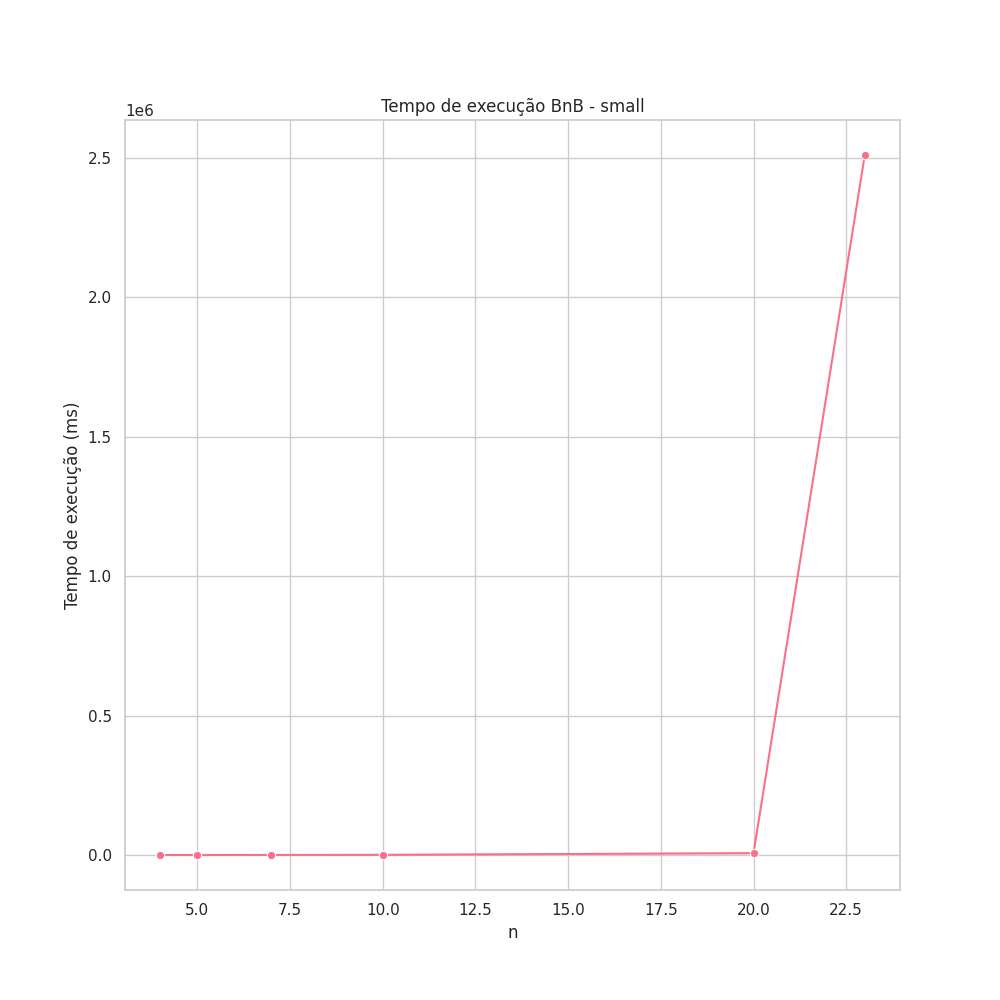
\includegraphics[width=\linewidth]{img/bnb_time_small.png}
        \caption{Tempo de execução em \(\mu s\) (pequeno)}
        \label{fig:bnb_small}
    \end{minipage}
    \hfill
    \begin{minipage}[b]{0.48\linewidth}
        \centering
        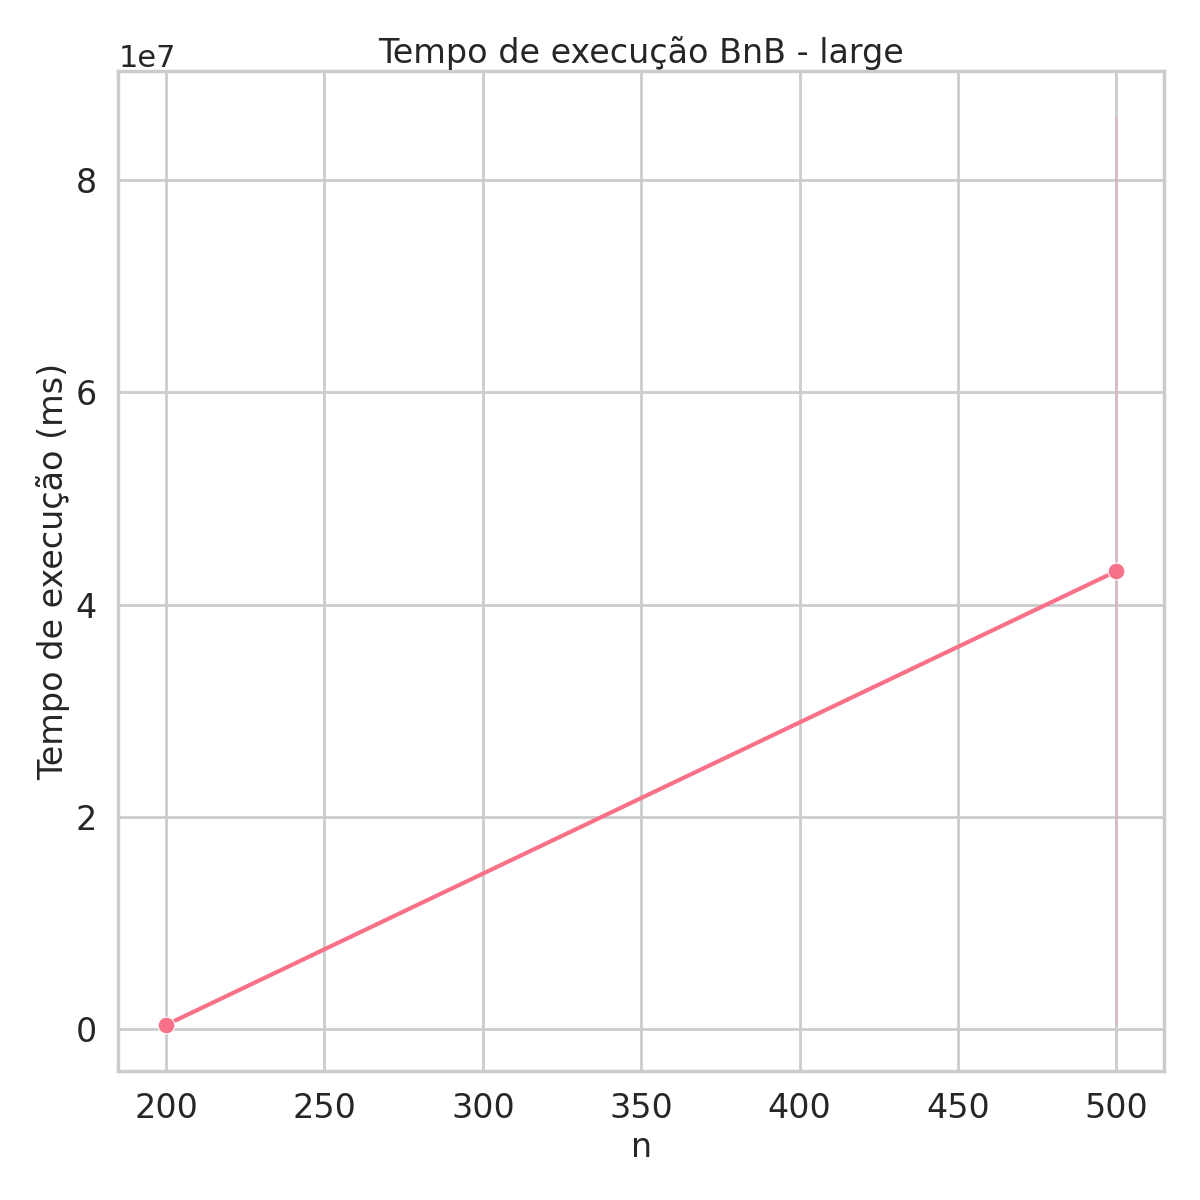
\includegraphics[width=\linewidth]{img/bnb_time_large.png}
        \caption{Tempo de execução em \(\mu s\) (grande)}
        \label{fig:bnb_large}
    \end{minipage}
\end{figure}

\vspace{-0.5cm}

O uso de \textbf{memória} foi condizente com o esperado, o uso de memória manteve-se abaixo de \texttt{12 MB}; o consumo estável de memória reflete uma implementação eficiente estrutura de dados. O aumento no tempo de execução deve estar relacionado à ordem dos itens, mas não houve impacto significativo no uso de memória.

\vspace{-0.5cm}


\begin{table}[H]
\centering
\caption{Intâncias, tamanho (n) e uso de memória em \textit{branch-and-bound} coletados com \texttt{getrusage}}
\begin{tabular}{|l|c|c||l|c|c|}
\hline
\textbf{Instância} & \textbf{n} & \textbf{Memória (KB)} & \textbf{Instância} & \textbf{n} & \textbf{Memória (KB)} \\
\hline
f3\_l-d\_kp\_4\_20 & 4 & 8480 & f4\_l-d\_kp\_4\_11 & 4 & 8452 \\
\hline
f9\_l-d\_kp\_5\_80 & 5 & 8516 & f7\_l-d\_kp\_7\_50 & 7 & 8608 \\
\hline
f1\_l-d\_kp\_10\_269 & 10 & 8872 & f6\_l-d\_kp\_10\_60 & 10 & 9288 \\
\hline
f2\_l-d\_kp\_20\_878 & 20 & 10912 & f10\_l-d\_kp\_20\_879 & 20 & 10976 \\
\hline
f8\_l-d\_kp\_23\_10000 & 23 & 10992 & knapPI\_14\_200\_1000\_1 & 200 & 11104 \\
\hline
knapPI\_1\_500\_1000\_1 & 500 & 11288 & knapPI\_2\_500\_1000\_1 & 500 & 11248 \\
\hline
\end{tabular}
\end{table}

\vspace{-0.5cm}

O algoritmo ainda possui uma característica notável, trata-se de um \textbf{algoritmo exato}, isto significa que a resposta encontrada é sempre ótima, mas , como visto, há um preço a se pagar no tempo de execução. Por exemplo, para uma instância de \(1000\) itens, não foi obtida resposta em menos de trinta minutos, o que pode ser indesejável. Contudo, ser um algoritmo exato significa que a \textbf{qualidade da resposta} é sempre ótima. Os dados do \texttt{CSV} garantem um \texttt{ratio}\(=1\) para todas as cargas de trabalho.

\subsection{Fully polynomial-time approximation scheme}

O esquema de aproximação permite a parametrização com \(\varepsilon\) do fator de aproximação; De tal maneira que, foi tomado \(\varepsilon \in \{0.1,0.25,0.5\}\), gerando três algoritmos aproximados com fatores de aproximação \(0.9, 0.75\) e \(0.5\) respectivamente.

O \textbf{tempo de execução} para os diferentes \(\varepsilon\)'s evidenciam uma correlação já esperada: O tempo de execução piora a medida que uma solução mais refinada é desejada. Ou seja, o algoritmo \(0.9\)-aproximativo é mais lento que o algoritmo \(0.5\)-aproximativo, embora com um limite de precisão mais apertado. Uma segunda observação importante, é que para casos pequenos, \(\varepsilon=0.25\) ou \(\varepsilon=0.5\) apresentaram pouca diferença no tempo; adiante será investiga a qualidade da solução.

\vspace{-0.5cm}

\begin{figure}[H]
    \centering
    \begin{minipage}[b]{0.48\linewidth}
        \centering
        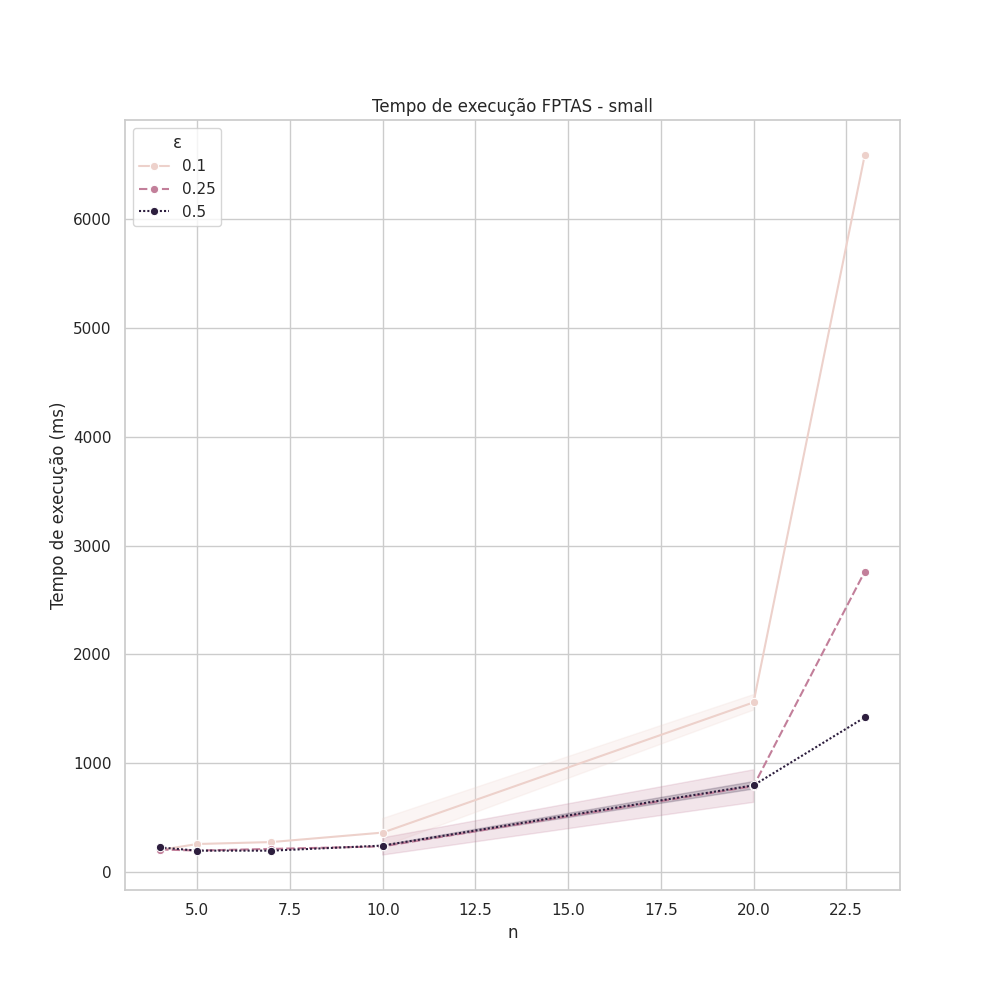
\includegraphics[width=\linewidth]{img/fptas_comparison_small.png}
        \caption{Tempo de execução em \(\mu s\), com 3 \(\varepsilon\)'s (pequeno)}
        \label{fig:fptas_small}
    \end{minipage}
    \hfill
    \begin{minipage}[b]{0.48\linewidth}
        \centering
        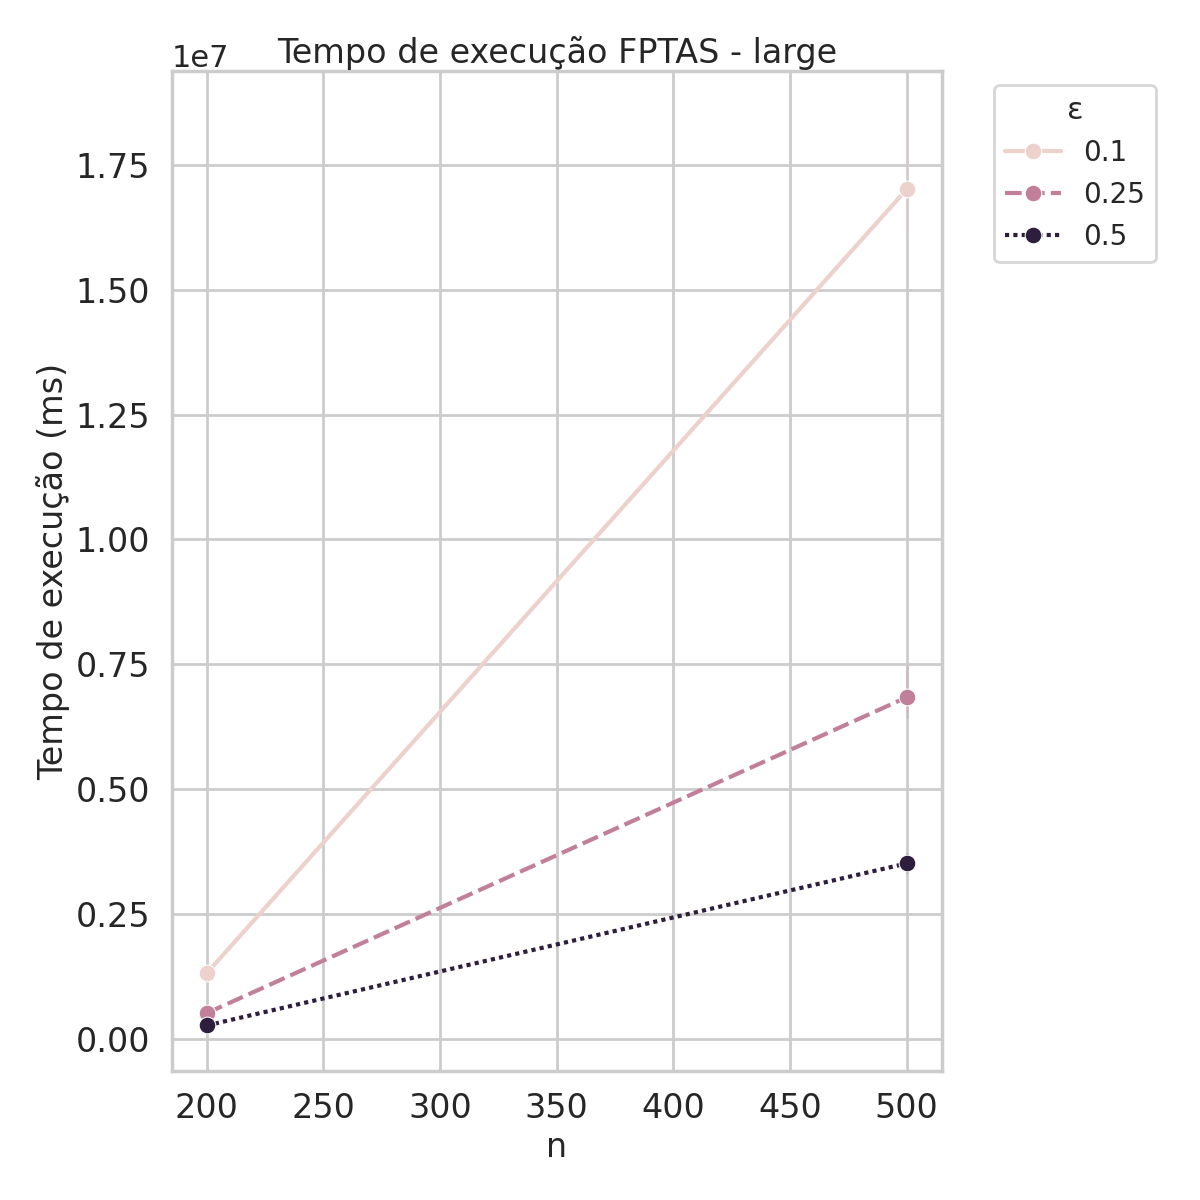
\includegraphics[width=\linewidth]{img/fptas_comparison_large.png}
        \caption{Tempo de execução em \(\mu s\), com 3 \(\varepsilon\)'s (grande)}
        \label{fig:fptas_large}
    \end{minipage}
\end{figure}

\vspace{-0.5cm}

A relação do uso de \textbf{memória} de acordo com o \(\varepsilon\) escolhido também foi esperada; Já que a complexidade de espaço para o problema da mochila no esquema de aproximação é \(\mathcal{O}\biggr(\frac{n^2}{\varepsilon}\biggr)\), isto é, para valores menores do parâmetro, o algoritmo deve trabalhar com uma escala mais refinada dos valores, aumentando o consumo de memória. As tabelas a seguir indicam os resultados experimentais. Em instâncias grandes como \texttt{knapPI\_3\_500\_1000\_1}, as dimensões de recursos utilizados foram discrepantes.

\vspace{-0.5cm}

\begin{table}[H]
\centering
\small
\caption{Uso de memória do FPTAS com \(\varepsilon=0.5\)}
\begin{tabular}{|l|c|r||l|c|r|}
\hline
\textbf{Instância} & \textbf{n} & \textbf{Memória (KB)} & \textbf{Instância} & \textbf{n} & \textbf{Memória (KB)} \\
\hline
f4\_l-d\_kp\_4\_11 & 4 & 8452 & f9\_l-d\_kp\_5\_80 & 5 & 8560 \\
\hline
f3\_l-d\_kp\_4\_20 & 4 & 8528 & f7\_l-d\_kp\_7\_50 & 7 & 8540 \\
\hline
f1\_l-d\_kp\_10\_269 & 10 & 8544 & f6\_l-d\_kp\_10\_60 & 10 & 8452 \\
\hline
f2\_l-d\_kp\_20\_878 & 20 & 8584 & f10\_l-d\_kp\_20\_879 & 20 & 8716 \\
\hline
f8\_l-d\_kp\_23\_10000 & 23 & 8864 & knapPI\_14\_200\_1000\_1 & 200 & 92624 \\
\hline
knapPI\_2\_500\_1000\_1 & 500 & 990988 & knapPI\_1\_500\_1000\_1 & 500 & 1017936 \\
\hline
knapPI\_3\_500\_1000\_1 & 500 & 1134368 & & & \\
\hline
\end{tabular}
\end{table}

\vspace{-0.7cm}

\begin{table}[H]
\centering
\small
\caption{Uso de memória do FPTAS com \(\varepsilon=0.25\)}
\begin{tabular}{|l|c|r||l|c|r|}
\hline
\textbf{Instância} & \textbf{n} & \textbf{Memória (KB)} & \textbf{Instância} & \textbf{n} & \textbf{Memória (KB)} \\
\hline
f4\_l-d\_kp\_4\_11 & 4 & 8560 & f9\_l-d\_kp\_5\_80 & 5 & 8540 \\
\hline
f3\_l-d\_kp\_4\_20 & 4 & 8560 & f7\_l-d\_kp\_7\_50 & 7 & 8528 \\
\hline
f1\_l-d\_kp\_10\_269 & 10 & 8440 & f6\_l-d\_kp\_10\_60 & 10 & 8520 \\
\hline
f2\_l-d\_kp\_20\_878 & 20 & 8636 & f10\_l-d\_kp\_20\_879 & 20 & 8624 \\
\hline
f8\_l-d\_kp\_23\_10000 & 23 & 9028 & knapPI\_14\_200\_1000\_1 & 200 & 175392 \\
\hline
knapPI\_2\_500\_1000\_1 & 500 & 1933536 & knapPI\_1\_500\_1000\_1 & 500 & 1989652 \\
\hline
knapPI\_3\_500\_1000\_1 & 500 & 2221020 & & & \\
\hline
\end{tabular}
\end{table}

\vspace{-0.7cm}

\begin{table}[H]
\centering
\small
\caption{Uso de memória do FPTAS com \(\varepsilon=0.1\)}
\begin{tabular}{|l|c|r||l|c|r|}
\hline
\textbf{Instância} & \textbf{n} & \textbf{Memória (KB)} & \textbf{Instância} & \textbf{n} & \textbf{Memória (KB)} \\
\hline
f4\_l-d\_kp\_4\_11 & 4 & 8460 & f9\_l-d\_kp\_5\_80 & 5 & 8608 \\
\hline
f3\_l-d\_kp\_4\_20 & 4 & 8536 & f7\_l-d\_kp\_7\_50 & 7 & 8460 \\
\hline
f1\_l-d\_kp\_10\_269 & 10 & 8708 & f6\_l-d\_kp\_10\_60 & 10 & 8536 \\
\hline
f2\_l-d\_kp\_20\_878 & 20 & 9016 & f10\_l-d\_kp\_20\_879 & 20 & 8968 \\
\hline
f8\_l-d\_kp\_23\_10000 & 23 & 9672 & knapPI\_14\_200\_1000\_1 & 200 & 409276 \\
\hline
knapPI\_2\_500\_1000\_1 & 500 & 4762812 & knapPI\_1\_500\_1000\_1 & 500 & 4902560 \\
\hline
knapPI\_3\_500\_1000\_1 & 500 & 5482992 & & & \\
\hline
\end{tabular}
\end{table}

Uma das dimensões da \textbf{programação dinâmica} do esquema de aproximação é a \textbf{soma dos valores dos itens}. Quanto maior a soma, mais estados de programação dinâmica são necessários, isso justifica resultados diferentes em memória para números de itens iguais, mas também apresenta impacto no tempo de execução.

\begin{figure}[H]
    \centering
    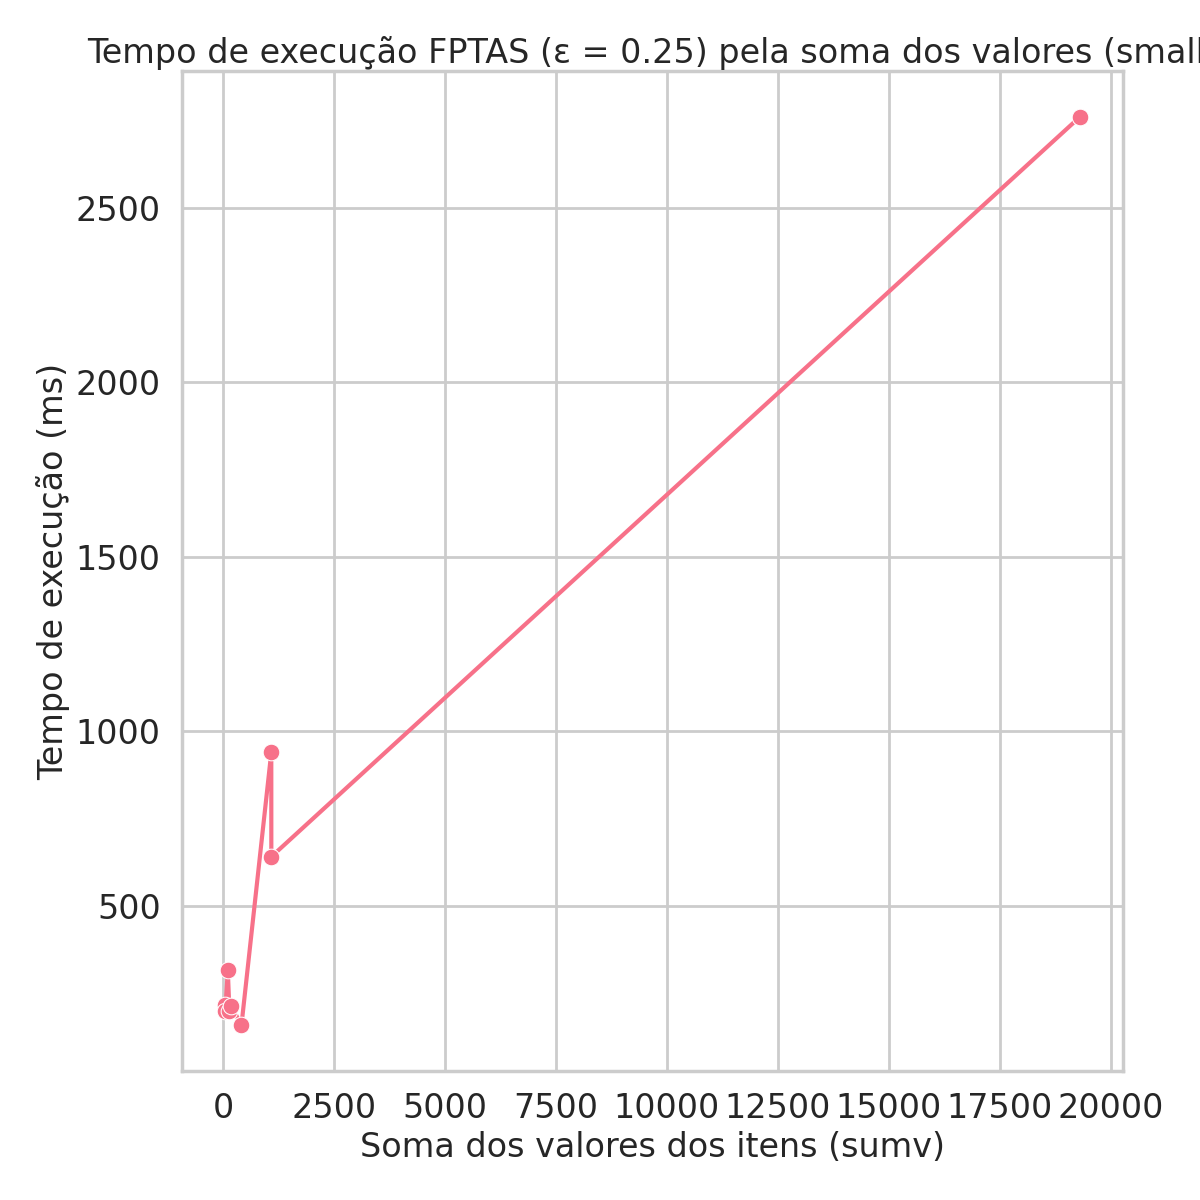
\includegraphics[width=0.48\linewidth]{img/fptas_eps_025_time_vs_sumv_small.png}
    \caption{Tempo de execução em \(\mu s\) de FPTAS em função da soma dos valores dos itens}
    \label{fig:enter-label}
\end{figure}

\vspace{-1cm}

\subsection{Algoritmo \(2\)-aproximado}

A técnica gulosa do algoritmo \(2\)-aproximado conferiu um tempo de execução praticamente linear e foi a mais rápida das três implementações. Abaixo os gráficos dos \textbf{tempos de execução} do algoritmo discutido.

\vspace{-0.3cm}

\begin{figure}[H]
    \centering
    \begin{minipage}[b]{0.48\linewidth}
        \centering
        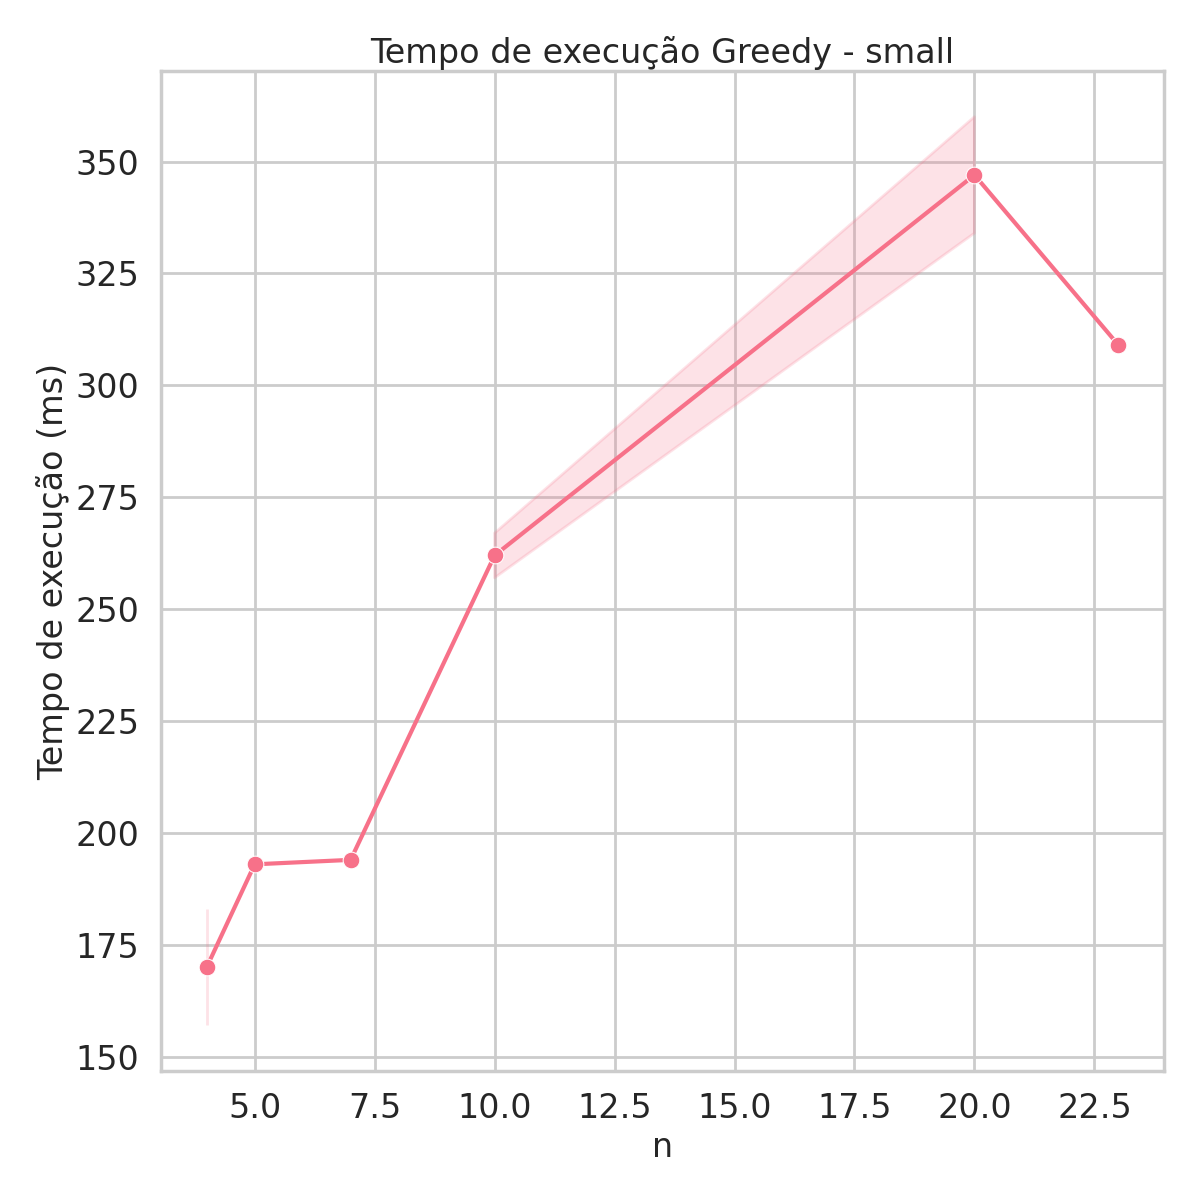
\includegraphics[width=\linewidth]{img/greedy_time_small.png}
        \caption{Tempo de execução em \(\mu s\) (pequeno)}
        \label{fig:fptas_small}
    \end{minipage}
    \hfill
    \begin{minipage}[b]{0.48\linewidth}
        \centering
        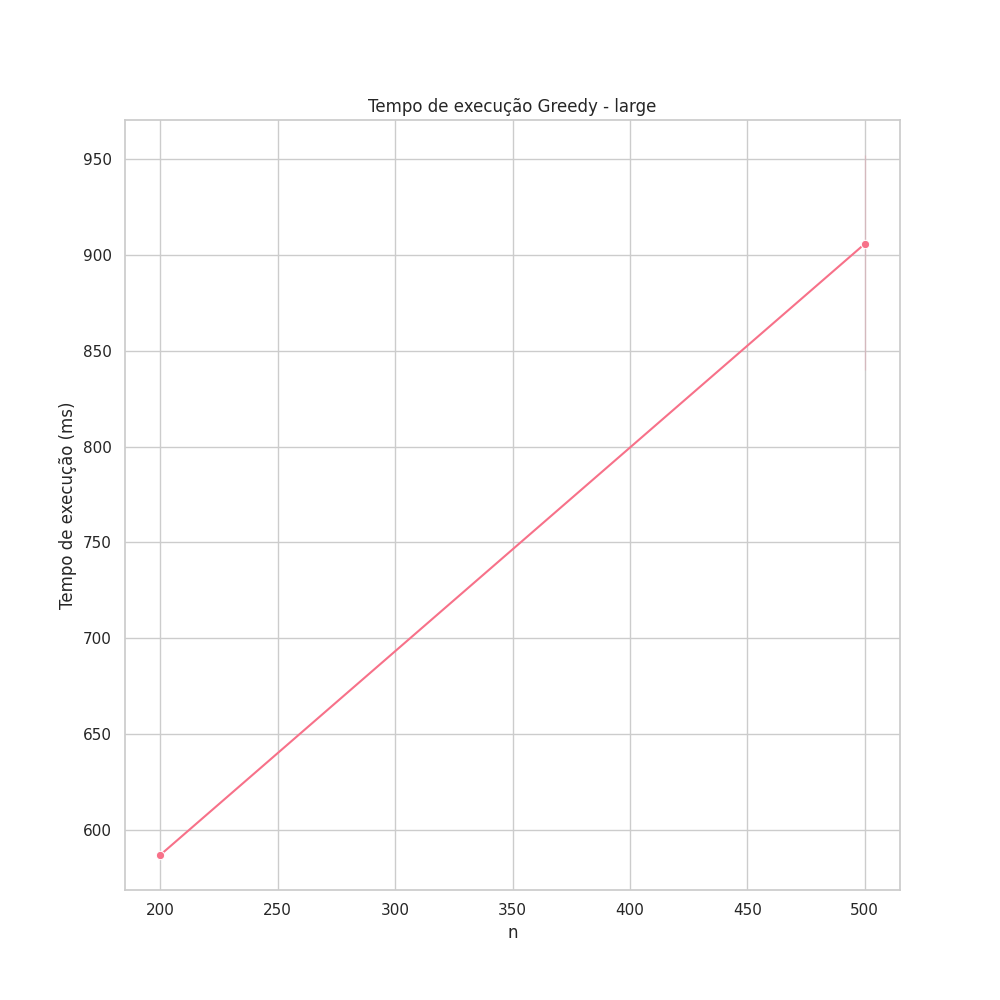
\includegraphics[width=\linewidth]{img/greedy_time_large.png}
        \caption{Tempo de execução em \(\mu s\)(grande)}
        \label{fig:fptas_large}
    \end{minipage}
\end{figure}
\vspace{-0.5cm}

O uso de \textbf{memória} do algoritmo \(2\)-aproximado não cresce durante as execuções, independentemente do tamanho da entrada o uso se manteve na faixa de \texttt{8500 KB}, indicando uma qualidade interessante do algoritmo que não tem nenhum tipo de estrutura de programação dinâmica ou recursiva .

\vspace{-0.5cm}

\begin{table}[H]
\centering
\caption{Uso de memória do algoritmo guloso 2-aproximado}
\begin{tabular}{|l|r|r||l|r|r|}
\hline
\textbf{Instância} & \textbf{n} & \textbf{Memória (KB)} & \textbf{Instância} & \textbf{n} & \textbf{Memória (KB)} \\
\hline
f4\_l-d\_kp\_4\_11      & 4   & 8480 & f3\_l-d\_kp\_4\_20      & 4   & 8472 \\
\hline
f9\_l-d\_kp\_5\_80      & 5   & 8432 & f7\_l-d\_kp\_7\_50      & 7   & 8456 \\
\hline
f6\_l-d\_kp\_10\_60     & 10  & 8456 & f1\_l-d\_kp\_10\_269    & 10  & 8480 \\
\hline
f2\_l-d\_kp\_20\_878    & 20  & 8368 & f10\_l-d\_kp\_20\_879   & 20  & 8560 \\
\hline
f8\_l-d\_kp\_23\_10000  & 23  & 8544 & knapPI\_14\_200\_1000\_1 & 200 & 8720 \\
\hline
knapPI\_1\_500\_1000\_1 & 500 & 9056 & knapPI\_2\_500\_1000\_1 & 500 & 8712 \\
\hline
knapPI\_3\_500\_1000\_1 & 500 & 8876 &                              &     &      \\
\hline
\end{tabular}
\end{table}

\vspace{-0.5cm}

\subsection{Análise comparativa entre os algoritmos}

Está claro que, cada um dos algoritmos responde o problema da mochila a sua maneira. Os gráfico a seguir são visualizações do tempo de execução de forma comparativa entre as implementações.

A solução exata tem \textbf{tempo de execução} maior que todas as outras implementações. A escolha do parâmetro \(\varepsilon\) para o esquema tem impactos no tempo do algoritmo, mas ainda não ultrapassa a técnica de \textit{branch-and-bound}, então é possível ter um fator de aproximação muito próximo do ótimo com um tempo de execução menor, mas não há garantia da resposta ótima sempre. Para situações reais onde a própria coleta de dados pode ser imprecisa, algoritmos aproximativos como o do esquema de aproximação podem ser muito flexíveis e úteis. Para absolutamente todas as instâncias, a técnica gulosa teve o menor tempo de execução.
Os gráficos a seguir apresentam tais informações sobre os algoritmos. 

\begin{figure}[H]
    \centering
    \begin{minipage}[b]{0.48\linewidth}
        \centering
        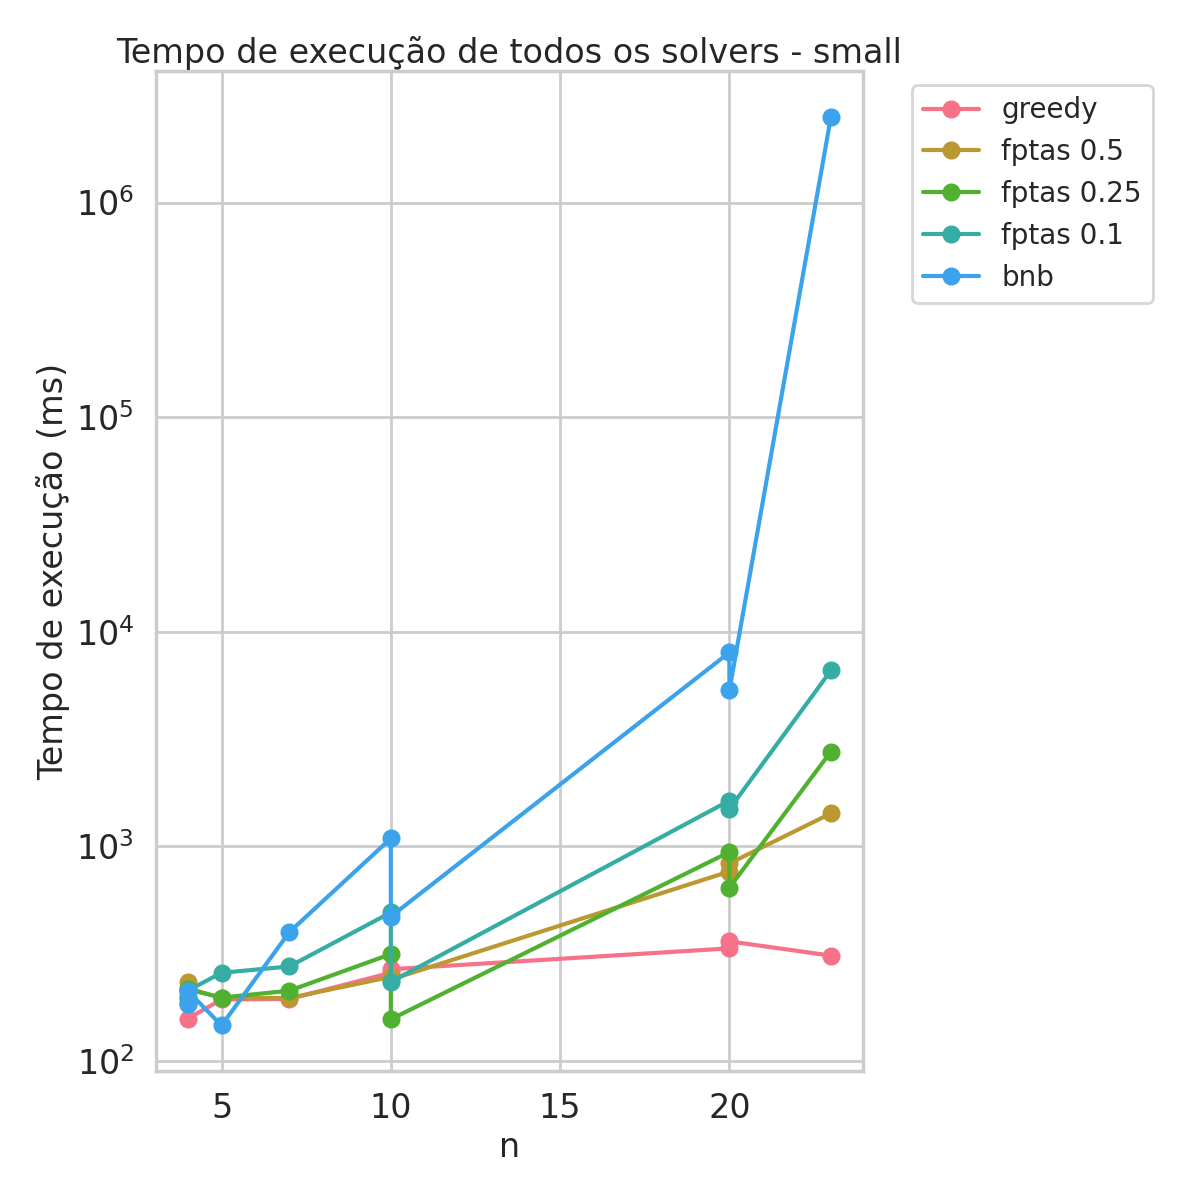
\includegraphics[width=\linewidth]{img/all_small.png}
        \caption{Comparação do tempo de execução em \(\mu s\) (pequeno)}
        \label{fig:fptas_small}
    \end{minipage}
    \hfill
    \begin{minipage}[b]{0.48\linewidth}
        \centering
        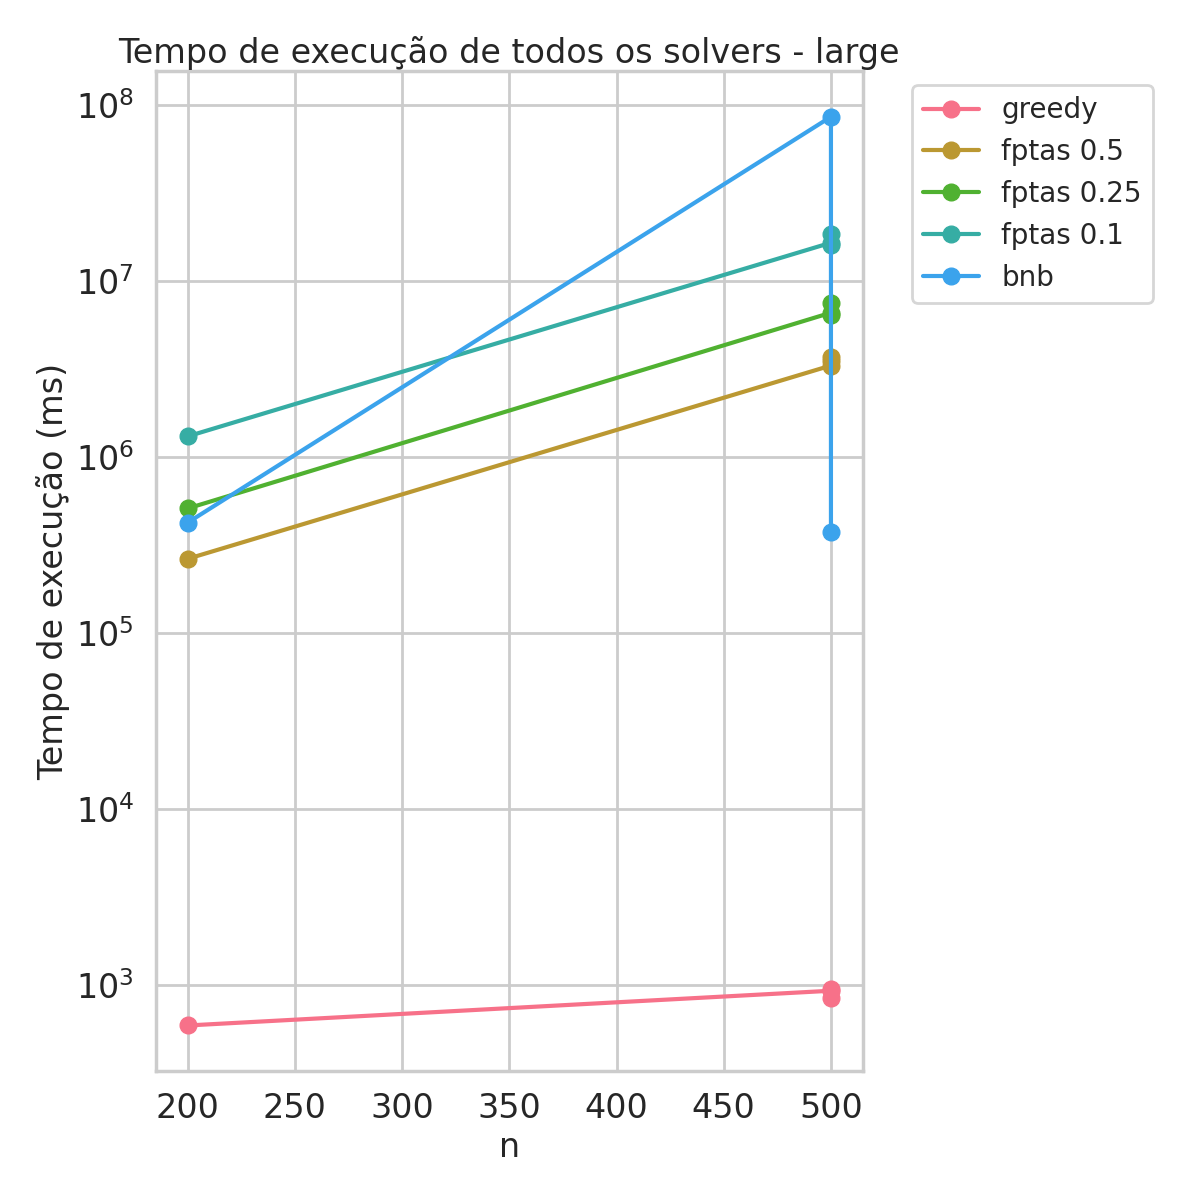
\includegraphics[width=\linewidth]{img/all_large.png}
        \caption{Comparação do tempo de execução em \(\mu s\)(grande)}
        \label{fig:fptas_large}
    \end{minipage}
\end{figure}

De acordo com as tabelas das sessões \(3.1\), \(3.2\) e \(3.3\), é possível uma análise de forma a comparar o \textbf{uso de memória} das abordagens implementadas. Para as instâncias pequenas, não houve tanta discrepância entre os resultados, mas o algoritmo guloso é a alternativa mais econômica em relação a recursos de armazenamento, de acordo com a tabela \(5\). Em contrapartida, \textit{fully polinomial-time aproximation scheme}, embora ofereça soluções aproximadas de alta qualidade, impõe um custo crescente de memória à medida que a precisão aumenta, o consumo de memória é substancial, vide tabela \(4\) para a intância de \(500\) itens. O algoritmo \textit{branch-and-bound} possui também consumo crescente de memória, embora seu ponto mais fraco ainda seja o alto tempo de execução.

\section{Conclusões}

Neste trabalho foram implementadas três abordagens para a solução do problema da mochila.

\section{Referências}

\begin{thebibliography}{1}

\bibitem{knp1}\textit{Dataset Large Scale 0/1 knapsack problems}. Disponível em: \url{https://www.kaggle.com/datasets/sc0v1n0/large-scale-01-knapsack-problems}. Acesso em: 02 de julho de 2025.

\bibitem{knp2}\textit{Instances of 0/1 Knapsack Problem}. Disponível em: \url{http://artemisa.unicauca.edu.co/~johnyortega/instances_01_KP/}. Acesso em: 02 de julho de 2025.

\bibitem{kt} KLEINBERG, Jon \& TARDOS, Éva. \textit{Algorithm Design}. Addison-Wesley, 2005.

\bibitem{levitin}LEVITIN, Anany. \textit{Introduction to The Design and Analysis of Algorithms}. 3rd edition. Addison-Wesley, 2012.

\bibitem{aprox} \textit{Mochila booleana aproximada}. IME-USP. Disponível em: \url{https://www.ime.usp.br/~pf/analise_de_algoritmos/aulas/mochila-aprox.html}. Acesso em : 04 de julho de 2025.

\end{thebibliography}

\end{document}
